%!TEX root = main.tex

\section{Shortcomings} % (fold)
\label{sec:shortcomings}
The finite difference time domain method is very good at approximating systems such as an electromagnetic wave. However there are a few areas where the model does not perform completely accurately. 

\subsection{Grid Size} % (fold)
\label{sub:grid_size}
The accuracy of the simulation depends both on the equations and approximations used in the mathematical representation of the wave and on the grid used to model and calculate that wave. The default size of the grid used here is 200 nodes long. That is, there are 200 electric field nodes and 200 magnetic field nodes used to calculate the field. Increasing this number would improve the accuracy and remove some of the artefacts shown previously. However, to do so would increase the time and processor load required for each simulation. This is a compromise that can be improved by optimising the code to take advantage of modern computing such as parallel computing and multi threaded calculations. These features are outside the scope of my knowledge.
% subsection grid_size (end)

\subsection{Ambiguous Dielectric Boundary} % (fold)
\label{sub:ambiguous_dielectric_boundary}

One example is when the wave encounters a dielectric boundary and is partially reflected from it. Consider the image in figure~\ref{fig:magneticgain}.

\begin{figure}[ht]
    \centering
    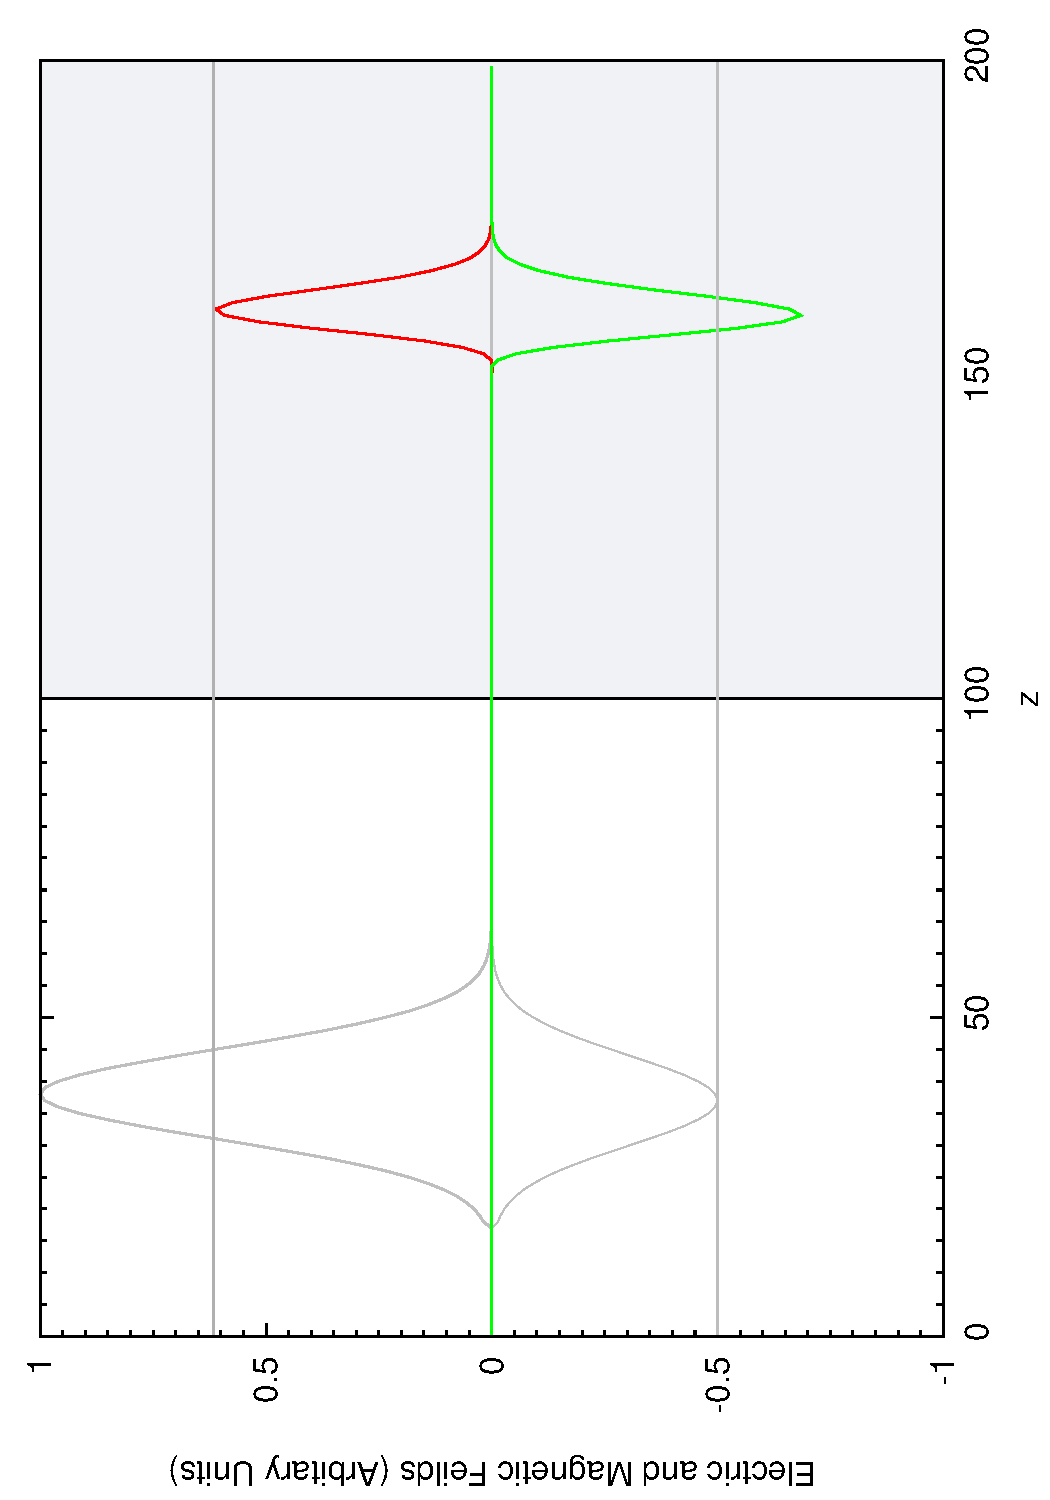
\includegraphics[angle=270, width=0.6\textwidth]{magneticgain.pdf}
    \caption{Several frames showing the wave after it has entered the dielectric material. Each image is 80 frames apart. The lossyness of the dielectric has been set to 0.01 which means the amplitude of the wave is 99\% of its previous value for each step of the simulation .}\label{fig:magneticgain}
\end{figure}

For this simulation, the lossy-less of the dielectric has been set to zero and a permittivity of 5.0 set. As can be seen, the electric field is reduced as would be expected. The magnetic field, however, has increased in magnitude since passing through the boundary. This does not make physical sense since the combined magnitude of the reflected (not shown) and the transmitted wave would be greater than the initial incident wave. This means that some energy has been added to the system despite no external source being present.

The reason for this discrepancy lies in the way that the nodes are arranged that make up the simulation area. There exist nodes that govern the size of the electric field and separate nodes for the magnetic field. These are arranged such that they alternate magnetic-electric-magnetic. This means that the boundary between the dielectric material and free space is not definite but somewhat ambiguous, as shown in figure~\ref{fig:dielectricnodes}.

\begin{figure}[ht]
	\centering
	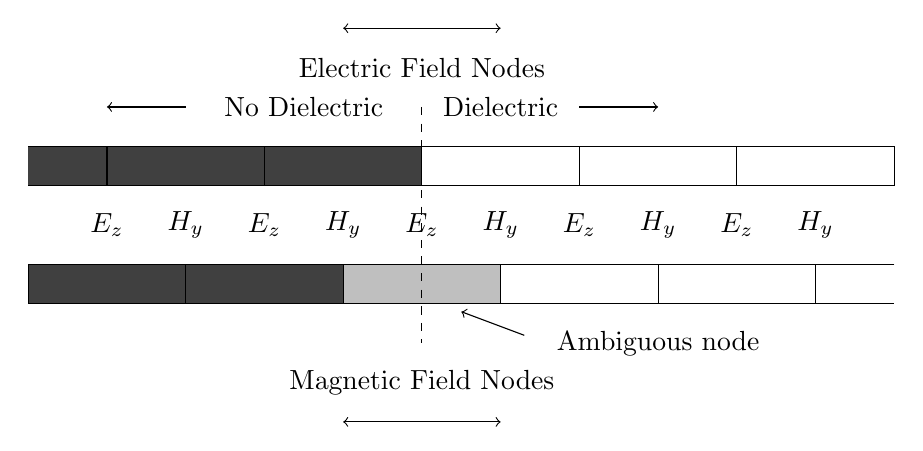
\begin{tikzpicture}
		\node (electric) at (4,2) {Electric Field Nodes};
		\draw [<->] (3,2.5) -- (5,2.5);
		\node (electric) at (4,-2) {Magnetic Field Nodes};
		\draw [<->] (3,-2.5) -- (5,-2.5);
		\node (electric) at (2.5,1.5) {No Dielectric};
		\draw [<-] (0,1.5) -- (1,1.5);
		\node (magnetic) at (5,1.5) {Dielectric};
		\draw [->] (6,1.5) -- (7,1.5);
		\node (1) at (0,0) {$E_z$};
		\node (2) at (1,0) {$H_y$};
		\node (3) at (2,0) {$E_z$};
		\node (4) at (3,0) {$H_y$};
		\node (5) at (4,0) {$E_z$};
		\node (6) at (5,0) {$H_y$};
		\node (7) at (6,0) {$E_z$};
		\node (8) at (7,0) {$H_y$};
		\node (9) at (8,0) {$E_z$};
		\node (10) at (9,0) {$H_y$};
		\draw [fill=darkgray] (-1,1) -- (2,1) -- (2,0.5) -- (-1,0.5);
		\draw [fill=darkgray] (0,1) -- (2,1) -- (2,0.5) -- (0,0.5) -- cycle;
		\draw [fill=darkgray] (2,1) -- (4,1) -- (4,0.5) -- (2,0.5) -- cycle;
		\draw (4,1) -- (6,1) -- (6,0.5) -- (4,0.5) -- cycle;
		\draw (6,1) -- (8,1) -- (8,0.5) -- (6,0.5) -- cycle;
		\draw (8,1) -- (10,1) -- (10,0.5) -- (8,0.5) -- cycle;
		\draw [fill=darkgray] (-1,-1) -- (1,-1) -- (1,-0.5) -- (-1,-0.5) -- cycle;
		\draw [fill=darkgray] (1,-1) -- (3,-1) -- (3,-0.5) -- (1,-0.5) -- cycle;
		\draw [fill=lightgray] (3,-1) -- (5,-1) -- (5,-0.5) -- (3,-0.5) -- cycle;
		\draw (5,-1) -- (7,-1) -- (7,-0.5) -- (5,-0.5) -- cycle;
		\draw (7,-1) -- (9,-1) -- (9,-0.5) -- (7,-0.5) -- cycle;
		\draw (10,-0.5) -- (9,-0.5) -- (9,-1) -- (10,-1);
		\draw [dashed] (4,1.5) -- (4,-1.5);
		\node (magnetic) at (7,-1.5) {Ambiguous node};
		\draw [->] (5.3,-1.4) -- (4.5,-1.1);
	\end{tikzpicture}
	\caption{Arrangement of the nodes that are used to calculate the evolution of the electric and magnetic fields and the ambiguity because of this when a dielectric is modelled.\label{fig:dielectricnodes}}
\end{figure}

When the simulation is run, using this arrangement of nodes, the boundary causes these irregularities to start, in the form of strange behaviour in the way the update equations are handled. To understand what is happening, we need to consider the individual nodes around the boundary, as shown in figure~\ref{fig:dielectricnodes}. As the wave moves towards the dielectric, the leading edge crosses the boundary as the electric field nodes are concerned, and so the relevant equations cause transmitted and reflected waves to be generated in accordance to the properties of the dielectric being modelled. However, the wave has not yet reached the magnetic node that is closest to the boundary. This means that there is a component that exists only as an electric field. Clearly this is non physical since the electric and magnetic field essentially generate each other, but the simulation exists in this state for a finite time.

When the wave encounters the magnetic field, the update equations use the value from the corresponding electric field node to calculate the magnetic field, but since the electric field is greater at that point than would be expected, the resulting magnetic field is also greater than expected. As the wave continues into the dielectric material, the calculations continue as usual, but with this error included. Over the length of the wave, i.e.\ the time it takes to move entirely into the dielectric and create the resulting reflected wave, the effect of the initial error is exaggerated so that the magnetic field ends up growing to larger than its initial value. The size of this effect is dependant on the characteristics of the dielectric, but is generally of the order of 1.3 to 1.6 times larger.

The best way to overcome this problem would be to have the dielectric boundary lie exactly on an electric and a magnetic field node. Unfortunately this would require the number of nodes to be increased hugely resulting in impractical calculation times and processor load. Alternatively, the electric and magnetic nodes could be placed at the same spacial position so that a boundary could be placed covering both, simply by placing it at a point where there are two nodes. This however would result in a simulation area that is unable to be used with the finite difference time domain algorithm since there would be no past value of one of the fields that could be used to calculate a further step in time. Other methods do exist, but the FDTD is one of the best in terms of calculation number and flexibility and so others are outside the scope of this report.

A compromise between these idealised situations is more reasonable. Instead of forcing the dielectric boundary to exist only at a single location, and to still be able to apply the FDTD method to the system, the existing set-up can be adapted to make the boundary more ``fuzzy'' but also more symmetrical so that there is less danger of these sorts of errors developing. If the boundary point is treated as the average of the two nodes on either side, the dielectric will appear to make a more gradual change from free space to a finite permittivity. This is done by replacing the absolute definition of the permittivity across the boundary with one that takes into account this difference in location, as shown in equation~\ref{eq:averagedielec}.
\begin{align}
	E^{q+\frac{1}{2}}_z(m) &\approx \frac{E^{q+1}_z(m)+E^q_z(m)}{2} \label{eq:averagedielec}
\end{align}
% subsection ambiguous_dielectric_boundary (end)

\subsection{Dimensional Constraints} % (fold)
\label{sub:dimensional_constraints}
Finally, an obvious shortcoming of this model is that it represents only the single $z$ dimension. For real world purposes, the full three dimensions would be required. This would require generalising the update equations from section~\ref{sub:finite_differences}
% subsection dimensional_constraints (end)
% section shortcomings (end)

\section{Conclusion} % (fold)
\label{sec:conclusion}
This project was designed to investigate and build a program to implement the finite difference time domain algorithm to calculate an electromagnetic wave as it interacted with different systems. The program allows the setting of a system with definable boundaries, and the ability to add a dielectric and change the lossyness and relative permittivity of that dielectric and also the option to model different starting waves, from a single Gaussian to a travelling sine wave as well as a finite sinusoidal wave pulse and to initiate that wave from either a single static source, or use a TFSF boundary.

The FDTD method is an extremely powerful method for modelling a system of differential equations. This program implements only a very small number of features that would be possible using the mathematical representation of the waves. There are also numerous improvements that could be made regarding the code quality, techniques and efficiency, since to model more complex systems would increase the number of calculations and so the processor load required dramatically.

Overall, however, this program is successful in implementing an initial trial of the FDTD method, incorporating Yee's algorithm.
% section conclusion (end)
